\documentclass[12pt,a4paper,utf8x,titlepage]{report}
\usepackage [frenchb]{babel}
\usepackage[utf8]{inputenc}  
\usepackage[T1]{fontenc} 
% Pour pouvoir utiliser 
\usepackage{ucs}
\usepackage{textcomp}
\usepackage{graphicx}
\usepackage{keystroke}
\usepackage{amssymb}
\usepackage{amsmath}
%\usepackage{pifont}
\usepackage{url} % Pour avoir de belles url
\usepackage{geometry}
\usepackage{hyperref}


\usepackage {listings}% Pour mettre du code source
\lstset{language=sh}

% Pour pouvoir passer en paysage
\usepackage{lscape}

% Pour pouvoir faire plusieurs colonnes
\usepackage {multicol}

\usepackage{makeidx}% Pour crééer un index
\usepackage{graphicx}
\usepackage{fourier-orns} %logo comme \danger
\usepackage[cc]{titlepic} %rajouter le logo LoCD dans la page de garde
\usepackage{tocbibind}
\usepackage{wasysym} %emoticones

\usepackage{glossaries} % Créer un glossaire

\hypersetup{
  backref=true,
  %permet d'ajouter des liens dans...
  pagebackref=true,%...les bibliographies
  hyperindex=true, %ajoute des liens dans les index.
  colorlinks=true, %colorise les liens
  breaklinks=true, %permet le retour à la ligne dans les liens trop longs
  urlcolor= blue, %couleur des hyperliens
  linkcolor= blue, %couleur des liens internes
  bookmarks=true, %créé des signets pour Acrobat
  bookmarksopen=true,
  %si les signets Acrobat sont créés,
  %les afficher complètement.
  pdftitle={Manuel Utilisateur pour LoCD}, %informations apparaissant dans
  pdfauthor={MARGUERITE Alain\\ RINCE Romain},
  %dans les informations du document
  pdfsubject={LoCD}
  %sous Acrobat.
}
%Entête pied de page
%Définition des entêtes : 
\usepackage{fancyhdr}
\pagestyle{fancy}

\renewcommand{\chaptermark}[1]{\markboth{#1}{}} % Pour avoir le nom du chapitre et de la numérotation.
\renewcommand{\sectionmark}[1]{\markright{\thesection\ #1}}
\fancyhf{} \fancyhead[LE,RO]{\bfseries\thepage}
\fancyhead[LO]{\bfseries\rightmark}
\fancyhead[RE]{\bfseries\leftmark}
\renewcommand{\headrulewidth}{0.5pt}% Pour le trait horizontal.
\addtolength{\headheight}{0.5pt}
\renewcommand{\footrulewidth}{0pt}
\fancypagestyle{plain}{ \fancyhead{}
\renewcommand{\headrulewidth}{0pt}} 


% Définition des pieds de pages : on veut un trait horizontal avec le numéro de page. 
\fancyfoot[C]{\thepage}%numéro de page
\renewcommand{\footrulewidth}{0.5pt} %trait horizontal pied de page


\makeindex


%%%% debut macro pour enlever le nom chapitre %%%%
\makeatletter
\def\@makechapterhead#1{%
  \vspace*{50\p@}%
          {\parindent \z@ \raggedright \normalfont
            \interlinepenalty\@M
            \ifnum \c@secnumdepth >\m@ne
            \Huge\bfseries \thechapter\quad
            \fi
            \Huge \bfseries #1\par\nobreak
            \vskip 40\p@
}}

\def\@makeschapterhead#1{%
  \vspace*{50\p@}%
          {\parindent \z@ \raggedright
            \normalfont
            \interlinepenalty\@M
            \Huge \bfseries  #1\par\nobreak
            \vskip 40\p@
}}
\makeatother
%%%% fin macro %%%%



%Couverture 
\titlepic{
\includegraphics[scale=0.30]{img/logo}}
\title{Manuel Utilisateur pour Logiciel de Création de Diagrammes}
\author{MARGUERITE Alain\\ RINCE Romain}
\date{\today}


%\storeglosentry{hist}{name=histoire,description=aventure}
%\makeglossary
\newglossaryentry{titre}{name=TITLE,description={Paramètre à fournir dans le fichier d'entrée pour donner un titre à votre diagramme.}}
\newglossaryentry{sous titre}{name=SUBTITLE,description={Paramètre à fournir dans le fichier d'entrée pour donner un sous titre à votre diagramme.}}
\newglossaryentry{note}{name=NOTE,description={Paramètre à fournir dans le fichier d'entrée pour fournir une note.}}
\newglossaryentry{metad}{name=Meta données,description={Informations à fournir en plus des données statistiques en elles mêmes (titre, note, \dots)}}
\newglossaryentry{unix}{name=Unix,description={Le système Unix est un système d'exploitation multi-utilisateurs, multi-tâches, ce qui signifie qu'il permet à un ordinateur mono ou multi-processeurs de faire exécuter simultanément plusieurs programmes par un ou plusieurs utilisateurs. }}
\begin{document}
\makeglossaries

\maketitle




\clearpage

\tableofcontents

\clearpage

% Pour avoir un interligne de 1,5

\section{Introduction et objectifs}
\label{chap:fichDonnees}
\subsection{Avis au lecteur} 
Ce manuel est destiné à un public désirant utiliser le logiciel GT. C'est à dire depuis son installation jusqu'à la génération du fichier au d'un fichier au format .ktr.Le manuel n'a pas pour objectif d'enseigner l'utilisation de cet outil. Les auteurs recommandes l'ouvrage suivant pour un tel apprentissage : \cite{kiwi}.

\subsection{Présentation du logiciel GT}
GT permet la génération automatique ou manuel de de systèmes temps réel.  L'outil est dédié est uniquement utilisable en mode console.

\section{Votre première simulation}
\sectionmark{1\up{ère} sim}
\subsection{Introduction}
Ce chapitre va vous permettre de réaliser une vote premierès simulation pour la validation de systèmes temps réel en moins de 2 minutes  \smiley ! Voici le résultat que vous obtiendrez au terme : 
\begin{figure}[htbp]
  \centering
 % 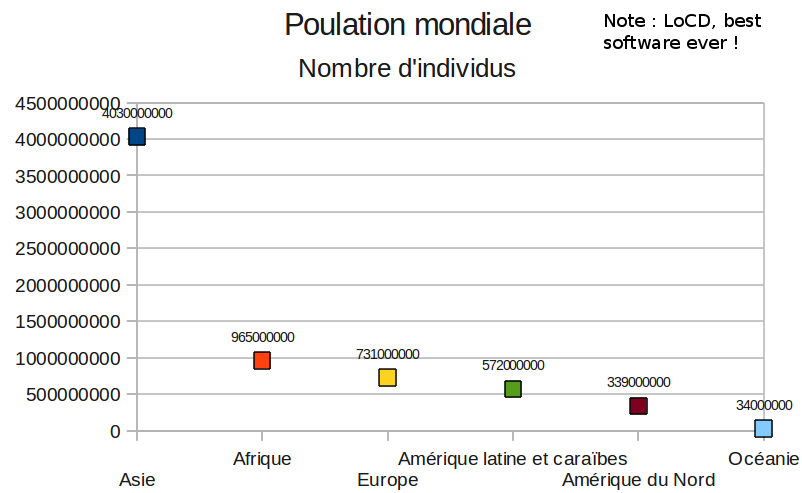
\includegraphics[scale=0.60]{img/diagrammenuages}
  \caption{Fichier .ktr}
  \label{fig:dnuages}
\end{figure}

\subsection{1\up{ère} \'Etape : Génération des tâches avec GT} 
\index{Comment commencer}
Dans le dossier GT, entrez la commande suivante \verb+./GT+. On vous propose d'entrez un nom de fichier. Entrez un nouveau nom si vous voulez créer vos propres tâches, ou entrez cours\_RMBG si vous voulez utiliser un exemple déjà éxistant. Il vous sera  demandé par la suite quel type d'ordonnancement vous désirez utiliser. Tapez R pour Rate Monotonic-Background. 

\subsection{2\up{ème} \'Etape : Utilisation de Kiwi}
Placez vous dans le dossier ou est installé Kiwi. Tapez la commande suivante  : \verb+./kiwi &+. Une fois dans l'interface de Kiwi, cliquez sur Open. Allez ouvrir votre fichier .ktr se trouvant dans le dossier ou est installé GT. Cliquez sur l'îcone Play. Voila ce que vous obtenez :  
\begin{figure}[htbp]
  \centering
 % 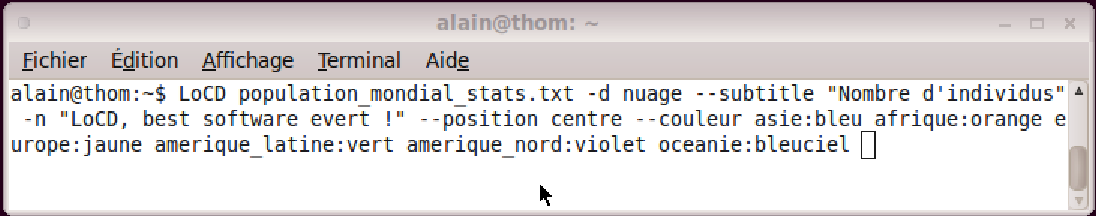
\includegraphics[scale=0.40]{img/ecommandes}
  \caption{Exemple d'utilisation de GT}
  \label{fig:commandes}
\end{figure} 


Et voilà avez crée votre première simulation pour la d'un systèmes temps réel  ! Si vous avez rencontrez des difficultés au cours de ce chapitre, vous pouvez vous référer aux différentes parties de ne manuel qui détaille chaque étapes en détail.

\section{Installation et configuration}

\subsection{Configuration nécessaire}
\label{sec:conf}
\index{Configuration requise}
\danger : GT est un outil open source dédié uniquement aux systèmes d'exploitation linux. Il n'existe pas encore de version pour Windows et MAC OS. L'installation requière des connaissances dans la manipulation de commandes shell. L'ouvrage suivant est une référence dans ce domaine : \cite{Nutshell}    

\subsection{Installation}
\label{sec:install}
Rendez vous sur \url{http://www.GT.org}. La rubrique «Download» vous proposera une archive de type tar.gz pour différentes distributions (solaris, Linux 32 Bit, Linux 64 Bit, \dots ). Le téléchargement terminé, décompressez l'archive dans le dossier où vous désirez installer GT. Placez vous dans ce dossier et tapez la commande \verb+java -jar GT+. GT est maintenant installé sur votre ordinateur \smiley !!  



\chapter{Utilisation du logiciel grâce à l'interface}\label{chap:usegraph}
  \begin{figure}[htbp]
    \centering
    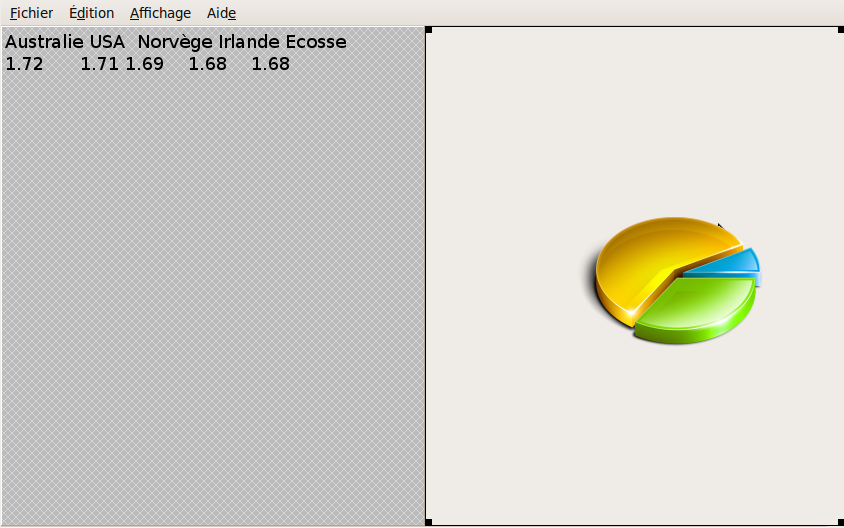
\includegraphics[scale=0.40]{img/soft}
    \caption{Apparence graphique de LoCD}
    \label{fig:apgraph}
  \end{figure}
Pour les utilisateurs peu à l'aise avec l'utilisation des commandes unix, LoCD propose un interface graphique. Bien qu'encore en developpement, cette interface permet de reprendre la plupart des fonctionalités disponibles en lignes de commandes. 
%\clearpage

%%%%%%%%%%%%%%%%%%%%%%%%%%%%%%%%%%%%%%%%%%%%%%%%%%%%%%%%%%%%%%%%%%%%%%%%%

\section{Lancement de l'application graphique}
\label{sec:lancegraph}
Si vous n'avez pas encore installé LoCD sur votre ordinateur, rendez vous à la section \ref{sec:install}. Une fois l'installion complète, il ne reste plus cliquer sur l'executable. Celui ci se trouve à l'emplacement : \verb+/.../LoCD_folder/bin/Locd+. Si un problème à lieu à ce stade, vérifiez que nous avez bien les configurations requises (\ref{sec:conf}). Pour tout autres problèmes \href{mailto:LoCD_assistance@exemple.com}{envoyez nous un mail}.

\section{Utilisation de l'interface graphique}
Voici un bref descriptif des différentes opération proposée par l'interface graphique de LoCD
\subsection{Barre des menus}
Les opérations générales sont listées dans la bare des tâches.
 \paragraph{Fichier}
 \begin{itemize}
\item
Ouvrir : Charger un ficher de données.
\item
Enregistrer : sauvegarder au format «.locd».
\item
Enregistrer sous : préciser le nom de votre sauvegarde.
\item
Exporter : Enregistrer votre diagramme au format de votre choix (pdf ou png).
\item
Quitter : Fermer l'application LoCD.
 \end{itemize} 
 
 \paragraph{Edition}
Ce menu possède le même contenu du menu contextel :
  \begin{figure}[htbp]
    \centering
    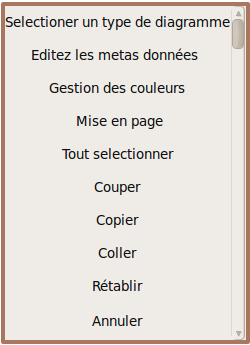
\includegraphics[scale=0.60]{img/menucont}
    \caption{Apparence du menu contextuel}
    \label{fig:menucont}
  \end{figure}

Les opérations : Selectioner un type de diagramme, Editez les metas données, Gestion des couleurs et Mise en page  effectuent les même règlages que ceus décrite dans le chapitre consacré à  l'utilisation par un terminal (\ref{chap:useterm}). Nous vous renvoyons à ce chapitre pour prendre connaissances de ces effets. La seule opération disponible exclusivement dans le menu edition est la rubrique Configuration par défault. Une nouvelle fenêtre s'ouvre et vous propose de régler des différents paramètres (couleurs, mise en page \dots) présents à la figure \ref{fig:dbatons}. 

\chapter{Fichier d'entrée}
\label{chap:fichDonnees}
L'utilisation de LoCD requière en entrée un fichier texte à la sytaxe précise. Ce fichier est composé de deux parties : Méta données et données.
\section{Partie Meta données du fichier d'entrée}
C'est ici que sont définies si besoins les informations décrivant le diagramme. Il est possble d'y préciser 3 sortes d'informations. 
\begin{enumerate}
\item
  Le titre 
\item
  Un sous titre
\item
  Une note
\end{enumerate}
Ces trois donnée doivent être décrite de la manière suivante : 
\begin{enumerate}
\item
  Une ligne par information 
\item
  Une ligne commence par  « > »
\item
  Un des trois mots clefs suivants : \begin{verbatim} TITLE SUBTITLE NOTE \end{verbatim}
\end{enumerate}
Un non respect du format qui va être décrit ci-après soulevera de l'erreur suivante  : 
\begin{figure}[htbp]
  \centering
  
\includegraphics[scale=0.40]{img/eformatfichier}
  \caption{Erreur : format}
  \label{fig:enbdonees}
\end{figure}
Si vous utlisez LoCD avec un terminal, le même texte de l'erreur apparaitra.



\section{Données}
Elles seront renseignées sur deux lignes. La première renseignera les étiquettes des données. Elles seront séparées par un ou des espaces (ou caractères de tabulation). Les valeurs seront sur la ligne suivantes. Les espaces (et\/ou caractères de tabulation) permettent de séparer deux étiquettes ou deux données :
\begin{verbatim}
Etiquette1 Etiquette2     Etiquette3 			Etiquette4
 \end{verbatim} 
 
Toutes les lignes ont une taille d’au maximum 80 colonnes. Dans le cas contraire l'erreur suivante sera relevée : 
\begin{figure}[htbp]
  \centering
  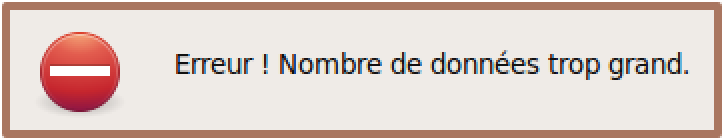
\includegraphics[scale=0.40]{img/enbdonnes}
  \caption{Erreur : nb données}
  \label{fig:enbdonees}
\end{figure}



\section{Exemple de fichier d'entrée}
Pour synthétiser les différents abordés dans ce chapitre voici un exemple de fichier d'entrée valide : 
\begin{verbatim}
  >TITLE: Les plus grands pays du monde pays (~2010)
  >SUBTITLE: En km²
  >Note: La France n'est que 42\up{ème}

  Russie      Canada 	   États-Unis    Chine 	    Brésil 
  17 098 242  9 984 670  9 629 091  	9 596 961  		8 514 877 km2 	
\end{verbatim}
sources \cite{wiki}

\chapter{Fonctionalités}
Nous détaillerons dans cette partie les différentes fonctionalités que propose l'outil. Des exemples illustrés et des \dots  
\section{Histogrammes}
Type de diagramme répendu, l'histogramme fait partie des diagrammes que LoCD peut générer. L'exmple ci-dessus illustre un résultat basique avec la configure par défaut de LoCD soit : 
\begin{itemize}
\item
Une unique couleur : bleu
\item
Absence de titre, sous titre et notes
\item
Représentation 2D
\end{itemize}
Pour changer cette configuration par défault, se référer au chapitre configuration% références !!!!!
\begin{figure}[htbp]
\centering
  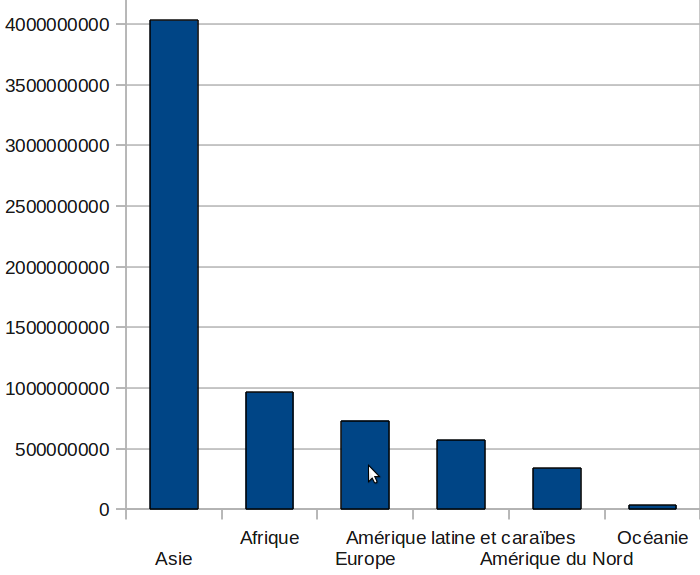
\includegraphics[scale=0.40]{img/diagrammebaton}
  \caption{Histogramme avec les paramètres par défaults}
  \label{fig:dbatons}
\end{figure}
  blah  blah  blah  blah  blah  blah  blah  blah  blah  blah  blah  blah  blah  blah  blah  blah  
\section{Diagrammes circulaires}
LoCD permet la création de diagrammes circulaires similaires  à celui présenté ci-dessous : 
\begin{figure}[htbp]
\centering
  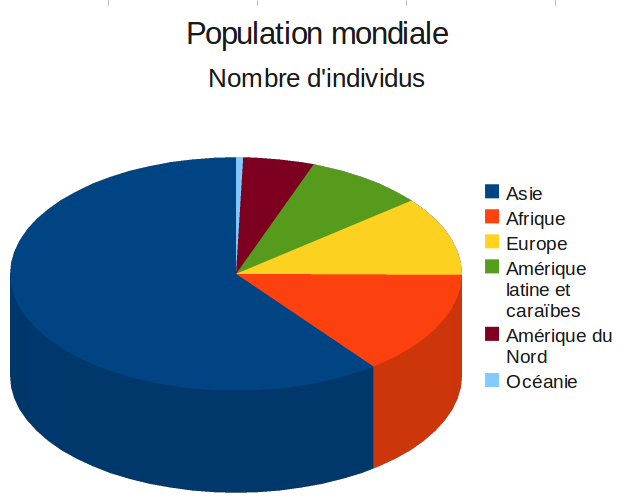
\includegraphics[scale=0.40]{img/diagrammecirculaire}
  \caption{Exemple avec un titre et un sous titre fournis dans les métas données.}
  \label{fig:dcirculaire}
\end{figure}
 blah  blah  blah  blah  blah  blah  blah  blah  blah  blah  blah  blah  blah  blah  blah  blah 
\clearpage
\section{Nuages de points}
\begin{figure}[htbp]
\centering
  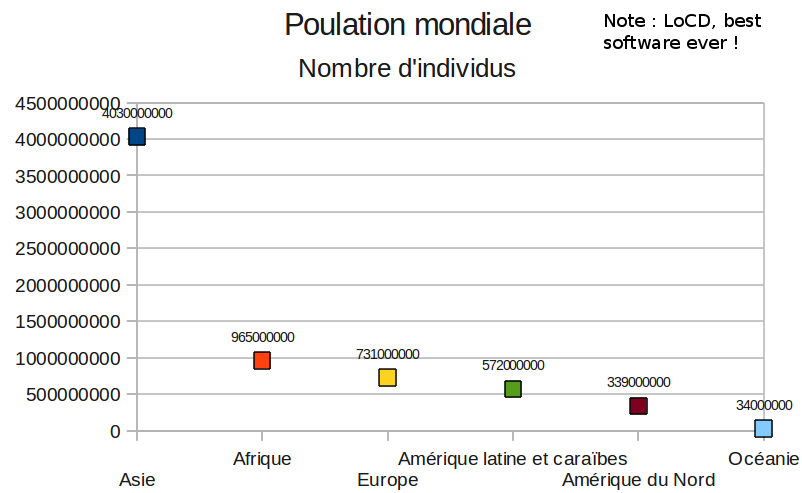
\includegraphics[scale=0.40]{img/diagrammenuages}
  \caption{Nuages de points avec toutes les méta données possible renseignées}
  \label{fig:dnuages}
\end{figure}  
  blah  blah  blah  blah  blah  blah  blah  blah  blah  blah  blah  blah  blah  blah  blah  blah 
  

\chapter{Utilisation console}
 
LoCD peut être utilisé uniquement en ligne de commande. Cette partie demandes des connaissances pré requises sur les commandes unix. En effet seul les fonctionalités de l'outil seront explicitées. La mecanisme des options est similaire à toute autres commandes unix. Pour plus de d'information sur les commandes unix, nous recommandons l'ouvrage suivant : \cite{linux}
%%%%%%%%%%%%%%%%%%%%%%%%%%%%%%%%%%%%%%%%%%%%%%%%%%%%%%%%%%%%%%%%%%%%%%
\section{Utilisation basique}
\label{sec:usebas}
La simple commande suivante générera un pdf avec d'un histogrammes avec les paramètres par défaut : % rajouter ref!!!!
\begin{verbatim}LoCD inputfile.txt\end{verbatim}Les choix du type de diagramme est possible grâce à l'option \verb+-t+ (ou \verb+--type+ ) suivit de : 
\begin{itemize}
\item
\verb+circulaire+ pour un diagramme circulaire.
\item
\verb+histogramme+ pour un histogramme.
\item
\verb+nuage+ pour un diagramme en nuage de points.
\end{itemize}
%%%%%%%%%%%%%%%%%%%%%%%%%%%%%%%%%%%%%%%%%%%%%%%%%%%%%%%%%%%%%%%%%%%%%%%%%%%%%%%%%%%%%%%%%%
\section{Gestion des méta données}
Une option pour chacune des méta données disponible (cf : ~\ref{chap:fichDonnees}) est définie :
\begin{itemize}
\item
\verb+-t+ ou \verb+--title+ pour afficher le titre.
\item
\verb+-s+ ou \verb+--subtitle+ pour afficher le sous titre.
\item
\verb+-n+ ou \verb+--note+ pour afficher le sous titre.
\end{itemize}
Si une de ces options est renseignée, il est possible de rajouter une valeur pour le paramêtre concerné. Par exemple : 
\begin{verbatim}
LoCD --title "Mon titre de diagramme" --subtitle "le sous" titre"
\end{verbatim} 
Dans le cas où l'une de ces options serait rajoutée ; et que aucune valeur ne lui est attribuée (en ligne de commande ou dans le fichier d'entrée) ; un avertissement apparaîtra à l'execution. Le diagramme n'aura pas de sous titre.\label{err:optmissing} % rajouter une ref!!!
%%%%%%%%%%%%%%%%%%%%%%%%%%%%%%%%%%%%%%%%%%%%%%%%%%%%%%%%%%%%%%%%%%%%%%%%%%%%%%%%%%%%%%%%%%

\section{Mise en forme reglages divers}
Le diagramme obtenu dans le cas d'une utilisation basique (~\ref{sec:usebas}) est stocké dans le dossier courant sous le nom de \verb+new_file.pdf+ et à les caractéristiques graphiques suivantes illustrée dans la figure :  ~\ref{fig:dbatons}.\\ Le changement du nom de ficher de sortie peut être modifier en rajoutant l'option \verb+-f outfilename+ ou dans sa version longue \verb+--filename+. 
\subsection{Couleurs}
\label{subsec:couleurs}
L'option \verb+-c+ (\verb+--couleur+) permet d'éditer la couleur de chaque données. Dans cette version LoCD propose une palette de 6 couleurs :
\begin{itemize}
\item
orange
\item
rouge
\item
vert
\item
bleu
\item
bleu ciel
\item
violet
\end{itemize}
Deux méthodes sont possibles :
\begin{enumerate}
\item
Faire suivre l'option d'un nom de couleur (listées ci-dessus). Le diagramme aura alors cette unique couleur.
\item
Faire suivre l'option du nom de la donnée puis d'un «couple» nom\_donnee:couleur séparé par le caractère \verb+:+. Une ou toutes les données peuvent être ainsi précisées. Dans tout autre cas, la couleur par défaut sera appliquée.
\end{enumerate}   
\subsection{Mise en page}
\label{subsec:misepage}
Dans la configuration par défault. Le diagramme est centrée dans une page de format A4 («au centre»). Le titre et le sous titre sont placés au dessus du diagramme (au nord»). La note elle, est placée à droite de des titres («nord est»). La figure \ref{fig:dnuages} est l'illustration de cette mise en page par défaut.
 

\section{Copyright}
	\paragraph{}
    Ce programme est un logiciel libre : vous pouvez le redistribuer ou
    le modifier selon les termes de la GNU General Public Licence tels
    que publiés par la Free Software Foundation : à votre choix, soit la
    version 3 de la licence, soit une version ultérieure quelle qu'elle
    soit.
	\paragraph{}
    Ce programme est distribué dans l'espoir qu'il sera utile, mais SANS
    AUCUNE GARANTIE ; sans même la garantie implicite de QUALITÉ
    MARCHANDE ou D'ADÉQUATION À UNE UTILISATION PARTICULIÈRE. Pour
    plus de détails, reportez-vous à la GNU General Public License.
	\paragraph	{}
    Vous devez avoir reçu une copie de la GNU General Public License
    avec ce programme. Si ce n'est pas le cas, consultez
 \cite{GNU}   
  \begin{figure}[htbp]
    \centering
    
\includegraphics{/home/alain/workspace/MiniP1/Rapport/img/gpl}
  \end{figure}  


% Pour finir l'interligne de 1,5
\printglossary

\listoffigures
\printindex



\appendix
%\bibliographystyle{AB_bib}
\bibliographystyle{alpha}
\bibliography{biblio.bib}

\end{document}

%Note : Installation package, décompressez les package dans un dossier. Changer la var set TEXINPUTS=/path/files
